%----------------------------------------------------------------------------
\chapter{Bevezetés}
\label{sec:intro}
%----------------------------------------------------------------------------

Féléves munkánk során egy perifériaillesztő modult valósítottunk meg System Verilog nyelven. Az illesztő az ARM\texttrademark Ltd. AMBA\texttrademark-APB rendszerbusza, és az I2C busz között teremt kapcsolatot. Ezen két buszt ismertetjük a továbbiakban.

\section{AMBA-APB}{
    Az Advanced Microcontroller Bus Architecture egy nyílt szabvány, amely chipen belüli kommunikációs összeköttetéseket definiál. Ennek a szabványnak része az Advanced Peripheral Bus (APB)\cite{APB} , amely alacsony sávszélességű, kis komplexitású, és minimális fogyasztású.

    \begin{table}[ht!]
        \begin{tabular}{l|p{0.7\textwidth}}
            \textbf{PCLK}       & Órajel, felfutó éle időzíti az összes átviteli ciklust. \\[3ex]
            \textbf{PRESETn}    & Reset, aktív-alacsony. \\[3ex]
            \textbf{PADDR}      & Címbusz, maximum 32 bit széles. \\[3ex]
            \textbf{PSELx}      & Slave-select, minden egységhez tartozik egy. Kiválasztja az adott slave egységet. \\[3ex]
            \textbf{PENABLE}    & Engedélyező jel, az átviteli ciklus második szakaszát jelzi. \\[3ex]
            \textbf{PWRITE}     & Irányjelző, magas értéke írást, alacsony értéke olvasást jelent. \\[3ex]
            \textbf{PWDATA}     & Adatbusz, maximum 32 bit széles, mindig a perifériabusz bridge hajtja. \\[3ex]
            \textbf{PRDATA}     & Adatbusz, maximum 32 bit széles, a slave egység hajtja az olvasási ciklusban.
        \end{tabular}
        \caption{Az APB busz jelei.}
        \label{tab:APBsig}
    \end{table}

    A busz jeleinek áttekintése után nézzünk egy írási ciklust a buszon. Minden átviteli ciklus két szakaszból áll, egy \emph{setup} és egy \emph{access} fázisból, ezen fázisok PCLK felfutó élére kezdődnek, ahogy az az \figref{APBtransfers} ábrán
    \footnote{Források: \tiny\\\url{http://infocenter.arm.com/help/topic/com.arm.doc.ddi0367b/graphics/apb_write_transfer_no_wait_states.svg}, \\ \url{http://infocenter.arm.com/help/topic/com.arm.doc.ddi0367b/graphics/apb_read_transfer_no_wait_states.svg}} megfigyelhető. A setup fázisban a híd eszköz (APB master) a PADDR buszra kiadja a címzett periféria címét, a PWRITE jelet az írásnak megfelelően magas értékűre állítja. A slave-hez tartozó PSEL vonalat is magas értékre állítja be, továbbá a PWDATA buszra kapuzza az írni kívánt adatot. Ebben a fázisban PENABLE alacsony értékű, így a slave eszköznek lehetősége van felkészülni az átvitelre. PCLK következő felfutó élére a PENABLE vonalat logikai 1 értékűre állítja, és ezzel a buszciklus végéig bezárólag a slave eszköz mintát vesz a PWDATA buszról, amivel lezárul az átvitel, PSEL, PWRITE és PENABLE visszaállításra kerül a master által.

    Az olvasás ciklus a vezérlőjeleket tekintve csak PWRITE értékében tér el. Ha az APB master olvasási ciklust kezdeményez, a PWRITE jelet logikai alacsony értékűre állítja a setup fázisban. Az access fázisban szintén kiadja a PENABLE jelet, mire a slave eszköz a megcímzett regiszterét a PRDATA buszra kapuzza. Az előzőekhez hasonlóan, a master vezérlőjeleket visszaveszi a ciklus befejeztével.
    \begin{figure}[ht!]
        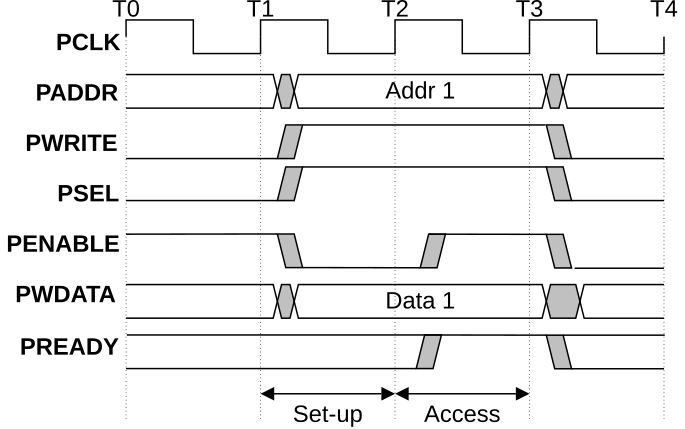
\includegraphics[width = 0.5\textwidth]{figures/apb_write_transfer_no_wait_states}
        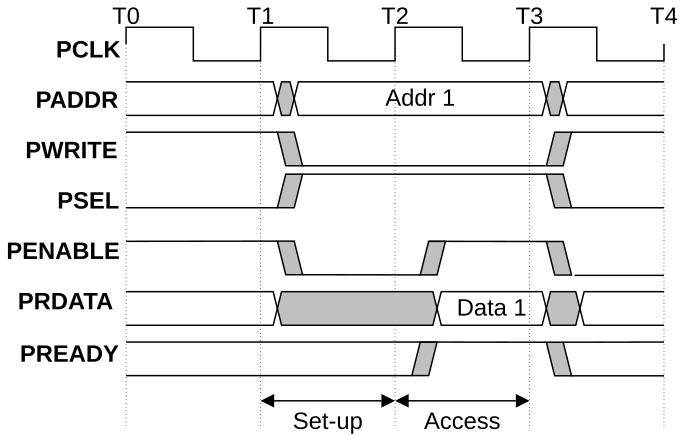
\includegraphics[width = 0.5\textwidth]{figures/apb_read_transfer_no_wait_states}
        \caption{Egy írási és olvasási ciklus időzítési viszonyai az APB buszon.}
        \label{fig:APBtransfers}
    \end{figure}
}

\section{I2C} {
    Az Inter-Integrated Circuit (vagy I2C, I\textsuperscript{2}C, esetleg IIC) egy multi-master, multi-slave, single-ended, félduplex soros kommunikációs busz.\cite{I2C}
    Két, nyitott kollektoros (open-drain) vezetéket használ a kétirányú kommunikációhoz, ezek az \emph{SDA} adatvonal és \emph{SCL} órajelvezeték. Fizikai kialakításból adódóan a vezetékeket ellenállásokon keresztül magas logikai (3V3, 5V, 1V8 stb.) feszültségre kell felhúzni. A buszra csatlakozó eszközök a vezetékeket "kényszeríteni" tehát csak lefelé tudják. Ez teszi lehetővé a multi-master struktúrához szükséges kiválasztást és arbitrációt, továbbá mivel különálló kiválasztó jelek (slave-select) nem állnak rendelkezésre, így az üzeneteket címezni kell. Egy üzenet felépítése látható az \figref{I2Cmessage} ábrán.\footnote{Forrás: \tiny\\\url{https://i2.wp.com/maxembedded.files.wordpress.com/2014/02/data-transfer-timing-diagram.png}}

    \begin{figure}[ht!]
        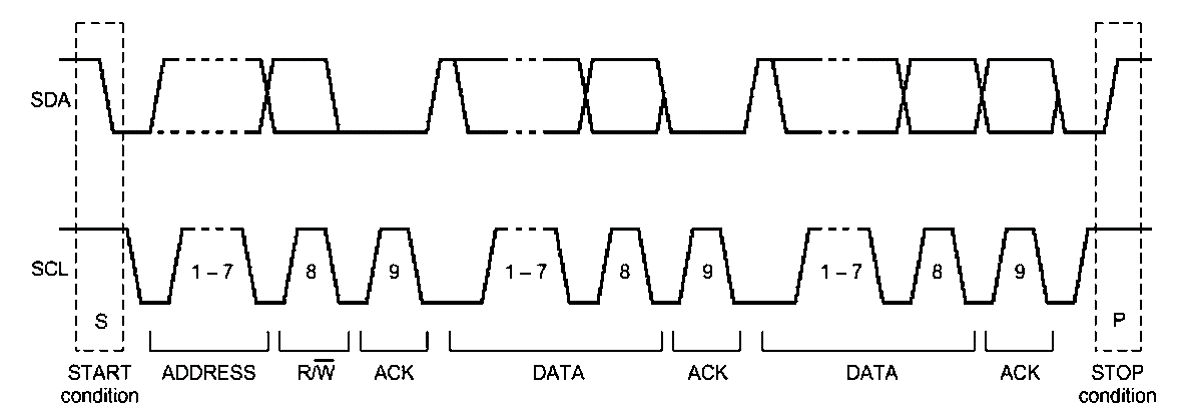
\includegraphics[width = \textwidth]{figures/i2ctiming}
        \caption{Az I2C busz időzítési diagrammja.}
        \label{fig:I2Cmessage}
    \end{figure}

    Az \emph{SCL} órajelet mindig a \emph{master} szolgáltatja a buszra csatlakozó eszközöknek.

    Minden üzenet a \emph{START} feltétellel (az SCL magas értéke mellett SDA lefutó éle) kezdődik és a \emph{STOP} feltétellel (az SCL magas értéke mellett SDA felfutó éle) végződik. Ezek speciális feltételek, az üzenet belsejében nem fordulhatnak elő, mivel SDA csak SCL alacsony értéke mellett változhat.

    A startbitet követi egy 7 bites címmező, amely a címzettet azonosítja, és egy \emph{R/\={W}} bit, amely írás esetén alacsony, olvasás esetén magas értékű. Ezután a küldő "elengedi" az adatbuszt, és a vevő, ha sikeres volt az átvitel, az adatbuszon a következő bit idejéig egy alacsony logikai értékű \emph{ACK} nyugtázó jelet ad az SDA vonalra. Ha ez megtörtént, a master további 8 órajelciklus alatt egy byte-nyi adatot kapuz az adatbuszra. Újabb nyugtázás esetén a byte átvitele befejeződött, és sikeres. A masternek lehetősége van további byteokat küldeni, szintén minden 8 bit adat után egy bit nyugtázással. Ha lezajlott a kívánt mennyiségű adat átvitele, a master kiadja a stopfeltételt, amely az üzenet végét jelenti.
}
